%光电检测技术第二章chapter2:光电检测技术基础
%author:Lang Xianli@hfut
%date: Sep 5, 2017
%\documentclass[10pt]{beamer}
\documentclass[trans]{beamer} %[trans]表示渐进效果pdf压缩打印
\usetheme[sectionpage=progressbar,subsectionpage=progressbar,numbering=counter,progressbar=head]{metropolis}
%numbering=定义页码显示方式;progressbar=定义进度条显示位置
\usepackage{appendixnumberbeamer}
%\usepackage{ctex}%中文字体支持宏包

\usepackage{booktabs}
\usepackage[scale=2]{ccicons}
\usepackage{array}    %支持表格固定宽度
\usepackage{xeCJK}  %中文字体支持宏包
\setCJKmainfont{fzlth.ttf} %方正兰亭黑
%\setsansfont{Ubuntu}
%\setmonofont{Ubuntu Mono}

\usepackage{pgfplots}
\usepgfplotslibrary{dateplot}

\usepackage{xspace}
\newcommand{\themename}{\textbf{\textsc{metropolis}}\xspace}

\title{第二章 光电检测技术基础}%Photoelectric Detection Technology
\subtitle{Photoelectric Detection Technology}
\date{\today}
\author{郎贤礼}
\institute{仪器学院  HFUT}
\titlegraphic{\hfill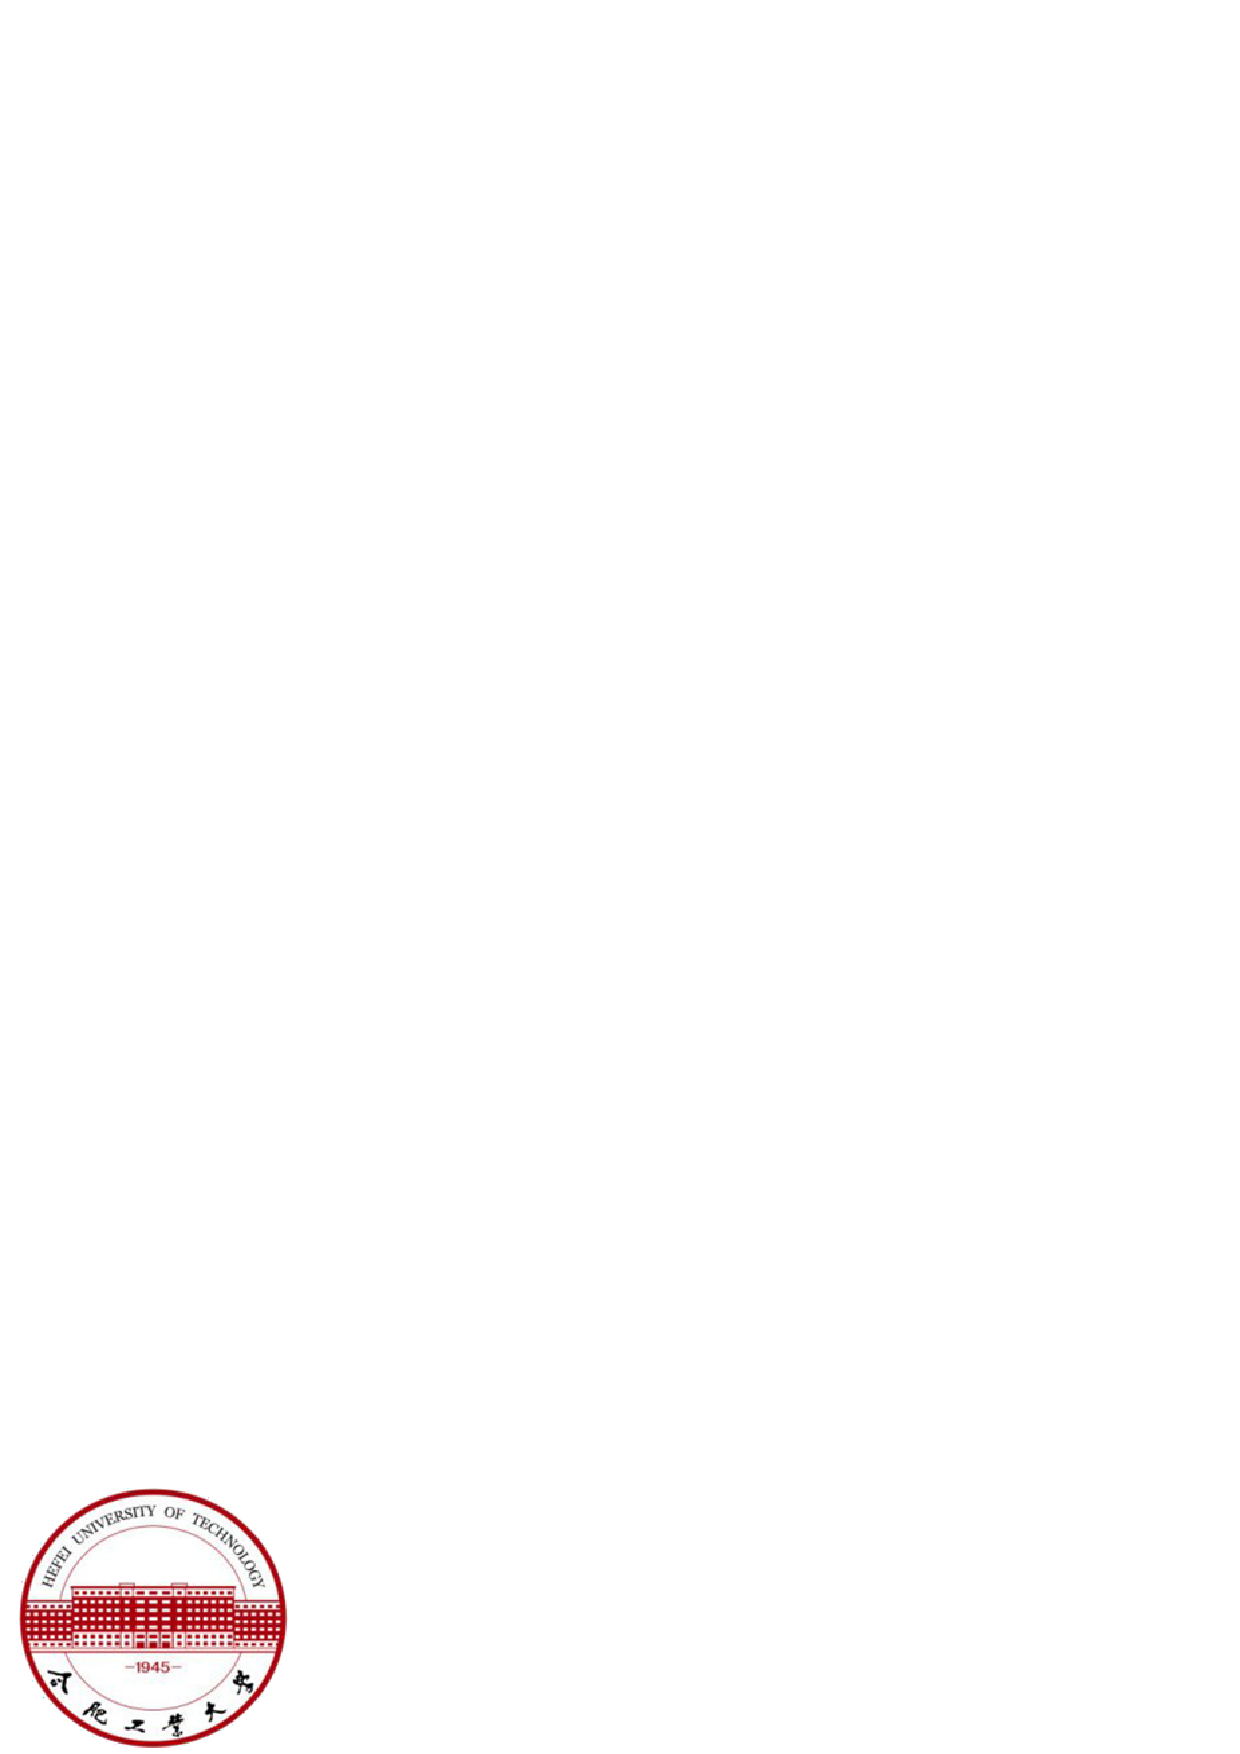
\includegraphics[height=2cm]{source/hfutlogo.png}}

\begin{document}

\maketitle

\begin{frame}{Table of contents}
  \setbeamertemplate{section in toc}[sections numbered]
  \tableofcontents[hideallsubsections]
\end{frame}

\section{光的基本性质}
\subsection{光的波粒二象性}

%%%%%%%%%%%%%%%%%%%%%%新一页演示文稿%%%%%%%%%%%%%%%%%%%%%%%%%%%%%%%%%%%%
\begin{frame}[fragile]{光的基本性质}
\begin{alertblock}{光的本质:}
	光是我们体验这个世界的基础。我们在黑暗中摸索,直到迎来黎明——而对于光本质的理解,我们也同样经历了同样痛苦的过程。

  然而,光的确是一种非常难以理解的事物:如果你用一台放大镜将一束光不断放大,你会看到什么?当然光的运动速度是极快的,但究竟是什么东西在运动?面对这样的问题,我们中的大部分人都会觉得难以回答。

  然而情况其实并没有那么糟糕,光的本质问题当然曾经在数百年里难倒了世界上最伟大的一些物理学家,但在过去的150年间,科学界在对光的本质研究方面取得了一系列的突破性进展,向世人揭示了光的神秘本质。

\end{alertblock}
	
	
\end{frame}

%%%%%%%%%%%%%%%%%%%%%%新一页演示文稿%%%%%%%%%%%%%%%%%%%%%%%%%%%%%%%%%%%%
\begin{frame}[fragile]{光的基本性质}
\begin{alertblock}{光的本质:}
	
	\end{alertblock}
	
	
  \begin{itemize}
    \item 牛顿微粒学说
        \begin{itemize}
           \item<2-| alert@2>[-] 根据光直线传播现象,对反射和折射做了解释
           \item<2-| alert@3>[-]  不能解释较为复杂的光现象:干涉、衍射和偏振
         \end{itemize}
    \item 波动理论
        \begin{itemize}
           \item<2-| alert@4>[-]  惠更斯、杨氏和费涅耳等
           \item<2-| alert@5>[-]  解释光的干涉和衍射现象
            \item<2-| alert@6>[-]  麦克斯韦电磁理论:光是一种电磁波
         \end{itemize}
    \item 光量子说:
        \begin{itemize}
           \item<2-| alert@7>[-]  1900年普朗克在研究黑体辐射时,提出辐射的量子论
           \item<2-| alert@8>[-]  1905年,爱因斯坦在解释光电发射现象时提出光量子的概念
           \item<2-| alert@9>[-]  光子的能量与光的频率成正比
           \item<2-| alert@10>[-] 光同时具有波和粒子的双重性质,即波粒二象性。
         \end{itemize} 
 \end{itemize}

  
  
\end{frame}
%%%%%%%%%%%%%%%%%%%%%%新一页演示文稿%%%%%%%%%%%%%%%%%%%%%%%%%%%%%%%%%%%%

\begin{frame}[fragile]{光的本质}

\alert{光的波粒二象性:}
\begin{center}
    \underline{不同条件下主要矛盾方面会发生转化}
\end{center}
%\overbrace{ }
\begin{columns}
        \begin{column}{0.5\textwidth}
        
        \begin{exampleblock}{波动性:}
        在反射、折射、干涉、衍射、色散等现象中,波动性往往成为主要矛盾方面,光便表现出像波。
      \end{exampleblock}
        \end{column}
        \begin{column}{0.5\textwidth}
        \begin{exampleblock}{粒子性:}
       在黑体辐射、光致发光、光电效应,以及其他一些有关光的产生和转化的现象中,粒子性往往成为主要矛盾方面,光便表现出像粒子。

      \end{exampleblock}
        
        \end{column}
        \end{columns}
        光的波、粒二重性的统一---德布罗意关系:
        \begin{equation}  \label{eq:db}
        E=h\nu
        \end{equation}
    
\end{frame}

%%%%%%%%%%%%%%%%%%%%%%新一页演示文稿%%%%%%%%%%%%%%%%%%%%%%%%%%%%%%%%%%%%

\begin{frame}[fragile]{光的本质}
\begin{alertblock}{光的电磁波谱:}
电磁场可以被看做是波动性和粒子性矛盾的统一体。它是一系列的波,同时又是光子的集合。		 

电磁波谱的频率范围很宽,涵盖了由宇宙射线到无线电波($10^2\sim10^{25}Hz$)的宽阔频域。光辐射仅是电磁波谱的一小部分,它包括的波长区域从几纳米到几毫米,即$10^{-9}\sim10^{-3}m$的范围。而且只有0.38~0.78μm的光才能引起人眼的视觉感,故称这部分光为可见光。
  
	\end{alertblock}
    \begin{figure}[htbp]
      \includegraphics[width=2.5in]{source/ch2/fg201mx.jpg}
      \caption{世界上第一张彩色照片,麦克斯韦拍摄,1861年}%\label{fig:2} 
  \end{figure}
\end{frame}




%%%%%%%%%%%%%%%%%%%%%%新一页演示文稿%%%%%%%%%%%%%%%%%%%%%%%%%%%%%%%%%%%%
\section{辐射度量与光度量}
\subsection{辐射度量}
\begin{frame}{光辐射度量}
光检测技术的任务是将光辐射转换成电能,从而获得光辐射的特征信息,因此需要了解辐射特征的定义。
    
    \begin{description}

      \item[\alert{辐射能$Q_e$}] 一种以电磁波的形式发射、传播或接受的能量。单位:焦耳[$J$]
      \item[\alert{辐射通量$\phi_e$}]
单位时间内通过一定面积发射、传播或接受的能量,又称辐射功率Pe,是辐射能的时间变化率。单位:瓦[W]
       \item[\alert{辐射强度$I_e$}]
点辐射源在给定方向上通过单位立体角内的辐射通量。单位:[W/Sr] 
      \item[\alert{辐射照度$E_e$}]
投射在单位面积上的辐射通量。单位:[W/m2]
      \item[\alert{辐射出射度$M_e$}]
扩展辐射源单位面积所辐射的通量(也称辐射本领)。单位:[W/m2]
      \item[\alert{辐射亮度$L_e$}]
辐射表面定向发射的辐射强度。单位:[W/m2.Sr]
     

  \end{description}
 \end{frame}

%%%%%%%%%%%%%%%%%%%%%%新一页演示文稿%%%%%%%%%%%%%%%%%%%%%%%%%%%%%%%%%%%%
\begin{frame}[fragile]{辐射度量}
 \begin{table}

 \caption{基本辐射度量的名称、符号和定义方程}
\label{table:2}
  \begin{center}
\begin{tabular}{ |m{1.8cm}|c|m{2.8cm}|m{1.8cm}|m{1.8cm}| } 
\hline
名称& 符号&定义方程 &单位&符号\\ 
\hline
辐射能& Q& 	& 	焦耳& 	J
 \\ 
\hline
辐射能密度& w&			& 焦耳/立方米& Jm-3
 \\ 
\hline
辐射通量辐射功率&P	&		&瓦特	&W \\
\hline
辐射强度&	I&		&瓦特/球面度&	Wsr-1 \\
\hline
辐射亮度&	L&	 	&瓦特/球面度平方米	&Wm-2 sr-1\\
\hline
辐射出射度	&M&	&	瓦特/平方米	W&m-2\\
\hline
辐射照度&	E&		&瓦特/平方米&	Wm-2\\
\hline
\end{tabular}
\end{center}
     
 \end{table}
\end{frame}
%%%%%%%%%%%%%%%%%%%%%%新一页演示文稿%%%%%%%%%%%%%%%%%%%%%%%%%%%%%%%%%%%%
\subsection{光度量}
\begin{frame}{光度量}
	
	\begin{alertblock}{光度量定义:}
	由于人眼的视觉细胞对不同频率的辐射有不同响应,对绿光最灵敏,对红光灵敏度最低,故用辐射度单位描述的光辐射不能正确反映人的亮暗感觉。 
光度单位体系是一套反映视觉亮暗特性的光辐射计量单位。
	\end{alertblock}
	
	\begin{itemize}
    
        \item 光度量和辐射度量的定义、定义方程是一一对应的。辐射度量下标为e,例如Qe,Φe,Ie,Me,Ee,光度量下标为v,Qv,Φv,Iv,Lv,Mv,Ev。


        \item 光度量只在可见光区(0.38~0.78μm)才有意义。
        \item 辐射度量和光度量都是波长的函数。 
    \end{itemize}
	
\end{frame}
%%%%%%%%%%%%%%%%%%%%%%新一页演示文稿%%%%%%%%%%%%%%%%%%%%%%%%%%%%%%%%%%%%
\begin{frame}{光度量的最基本单位}
    \begin{itemize}
        \item \alert{发光强度Iv:}
发出波长为555nm的单色辐射,在给定方向上的发光强度规定为1cd。单位:坎德拉(Candela)[cd],它是国际单位制中七个基本单位之一。
        \item \alert{光通量Φv:}
光强度为1cd的均匀点光源在1sr内发出的光通量。单位:流明[lm]。
        \item \alert{光照度Ev:}
单位面积所接受的入射光的量 ,单位:勒克斯[lx],相当于 1平方米面积上接受到1个流明的光通量。 

    \end{itemize}
    
\end{frame}

\section{半导体物理基础}
\subsection{固体物理基础}
%%%%%%%%%%%%%%%%%%%%%%新一页演示文稿%%%%%%%%%%%%%%%%%%%%%%%%%%%%%%%%%%%%
\begin{frame}{固体物理基础}
    \begin{itemize}
        \item \alert{晶体结构:}\\
            \begin{itemize}
            \item<2-| alert@2>[+] 晶态:原子周期排列、长程有序(微米量级) 
            \item<2-| alert@3>[+] 非晶态:原子排列短程有序、长程无序
            \item<2-| alert@4>[+] 准晶态:原子位置有序、但无周期性
        
                \end{itemize}
        \item \alert{晶格(lattice)原胞(Primitive cell)晶胞(cell)}:\\
                \begin{itemize}
            \item<2-| alert@5>[+] 原胞:体积最小的重复单元 a1, a2, a3

            \item<2-| alert@6>[+] 晶胞:结晶学上所取的重复单元a, b, c

                \end{itemize}
        \item \alert{空间点阵(布拉菲格子)}
    
        \begin{itemize}
            \item<2-| alert@7>[+] 基元--组成晶体的最小结构单元。
    把基元抽象成为一点,则晶体抽象成为空间点阵。\\
           \end{itemize}     

    \end{itemize}

\end{frame}
%%%%%%%%%%%%%%%%%%%%%%新一页演示文稿%%%%%%%%%%%%%%%%%%%%%%%%%%%%%%%%%%%%
\begin{frame}{一个检测的例子}
\begin{underline}晶体结构=基元+空间点阵
\end{underline}
 
  \begin{figure}[htbp] 
    \centering\includegraphics[height=2in]{source/ch2/fg202.png} 
    \caption{光电检测系统组成}\label{fig:joy}
    \end{figure} 
 
 \end{frame}
%%%%%%%%%%%%%%%%%%%%%%新一页演示文稿%%%%%%%%%%%%%%%%%%%%%%%%%%%%%%%%%%%%
\begin{frame}{空间点阵}
    

    \begin{alertblock}{布拉菲格子(空间点阵):}
    把空间点阵用三组不共面的             平行线连起来,形成的空间网格。               此时,又把阵点称为格点。
布拉菲格子(B格子)=空间点阵
    \end{alertblock}
    \begin{figure}[htbp] 
    \centering\includegraphics[height=2in]{source/ch2/fg203.png} 
    \caption{空间点阵}\label{fig:jy}
    \end{figure}  
\end{frame}


%%%%%%%%%%%%%%%%%%%%%%新一页演示文稿%%%%%%%%%%%%%%%%%%%%%%%%%%%%%%%%%%%%
\begin{frame}{空间点阵}
说     明
    \begin{enumerate}[(1)]
        \item <2-|alert@2> 基元中A、B可以是不同的原子,或相同的原子,但周围“  环境”不同。
        \item 每个基元用一个格点来表示。此格点选在基元的什么地方、代表几个原子并未限制。
        \item 每个基元内所含的原子数=晶体中原子的种类数。
        \item 布拉菲格子(B格子)的基本特征:各格点的情况(基元内涵和周围“  环境”)完全相同。
        \item 晶体结构的一种描述:带基元的B格子。
        \item  另一种描述:单式格子:晶体由一种原子组成。一个基元仅有一个原子,即一个原子由一个格点表示。
    \end{enumerate}


\end{frame}


%%%%%%%%%%%%%%%%%%%%%%新一页演示文稿%%%%%%%%%%%%%%%%%%%%%%%%%%%%%%%%%%%%
\begin{frame}{元胞,基矢和晶胞}
元胞和基矢
   

    \begin{itemize}
        \item 元胞:B格子中的最小重复区域。
         每个初级元胞只包含一个格点。
        \item 基矢:在B格子中任取一个格点为原点, 
       元胞的三个棱边为三个矢量$a_1$、$a_2$、$a_3$,其模分别为该方向的最小周期长度,这三个矢量$a_1$、$a_2$、$a_3$称为基矢 
        \item 基矢选定之后,B格子中的任一格点的位矢
        \begin{displaymath}
        \vec{R}_n= n_1\vec{a}_1+ n_2\vec{a}_2+ n_3\vec{a}_3
        \end{displaymath}
 $\vec{R}_n$称为格矢,是B格子的数学表示
    \end{itemize}
\end{frame}

%%%%%%%%%%%%%%%%%%%%%%新一页演示文稿%%%%%%%%%%%%%%%%%%%%%%%%%%%%%%%%%%%%
\begin{frame}{元胞,基矢和晶胞}
注意:
    \begin{enumerate}
            \item<2-| alert@2>[-] 基矢的选法并不唯一确定,(初基元胞内仅含一个格点)。
            \item<2-| alert@3>[-] 晶胞(惯用原胞):体积是初基元胞的几倍,能明显地反映晶格的周期性,又能明显地反映晶格的对称性。
    \end{enumerate}
    \begin{figure}[htbp] 
            \centering\includegraphics[width=4in]{source/ch2/fg204.png} \caption{基矢的选法并不唯一}
            \end{figure}
\end{frame}

%%%%%%%%%%%%%%%%%%%%%%新一页演示文稿%%%%%%%%%%%%%%%%%%%%%%%%%%%%%%%%%%%%
\begin{frame}{几种常见立方晶系结构}
结晶学中属于立方晶系的原胞,简立方sc,体心立方bcc和面心bcc立方。\\
            
    \begin{columns}
        \begin{column}{0.5\textwidth}
        
         \begin{figure}[htbp] 
            \centering\includegraphics[width=1.2in]{source/ch2/fg205.png} \caption{简立方}%\label{fig:3a} 
            \end{figure}
            \begin{figure}[htbp] 
            \centering\includegraphics[width=1.2in]{source/ch2/fg206.png} \caption{体心立方} 
            \end{figure}
        \end{column}
        \begin{column}{0.5\textwidth}
        \begin{figure}[htbp] 
            \centering\includegraphics[width=1.2in]{source/ch2/fg207.png} \caption{面心立方}%\label{fig:3a} 
            \end{figure}
        
        \end{column}
        \end{columns}        
           
            
\end{frame}


%%%%%%%%%%%%%%%%%%%%%%新一页演示文稿%%%%%%%%%%%%%%%%%%%%%%%%%%%%%%%%%%%%
\begin{frame}{金刚石结构与闪锌矿晶体结构}

    \begin{itemize}
        \item \alert{金刚石结构 Si Ge}\\每个原子周围有四个最邻近的原子,这四个原子处于正四面体的顶角上,任一顶角上的原子和中心原子各贡献一个价电子为该两个原子所共有,并形成稳定的共价键结构。
        \item \alert{金刚石结构结晶学原胞}\\
两个面心立方沿立方体空间对角线互相位移了四分之一的空间对角线长度套构而成。
        \item \alert{金刚石结构固体物理学原胞}\\
中心有原子的正四面体结构(相同双原子复式晶格)
        \item 闪锌矿结构固体物理学原胞
中心有原子的正四面体结构(双原子复式晶格)
        \item 与金刚石结构的区别:共价键具有一定的极性(两类原子的电负性不同),因此晶体不同晶面的性质不同。不同双原子复式晶格。
   \end{itemize}
\end{frame}
%%%%%%%%%%%%%%%%%%%%%%新一页演示文稿%%%%%%%%%%%%%%%%%%%%%%%%%%%%%%%%%%%%
\begin{frame}{金刚石结构与闪锌矿晶体结构}

    \begin{columns}
        \begin{column}{0.5\textwidth}
        
        \begin{exampleblock}{金刚石结构与闪锌矿晶体结构:}
        金刚石结构的区别:共价键具有一定的极性(两类原子的电负性不同),因此晶体不同晶面的性质不同。不同双原子复式晶格。
        
      \end{exampleblock}
             \begin{figure}[htbp] 
            \centering\includegraphics[width=1.75in]{source/ch2/fg208.png} \caption{金刚石结构}
            \end{figure}
        \end{column}
        \begin{column}{0.5\textwidth}
        \begin{exampleblock}{闪锌矿晶体结构:}
      半导体光电材料多为闪锌矿晶体结构,比如GaAs等。

      \end{exampleblock}
        \begin{figure}[htbp] 
            \centering\includegraphics[width=1.75in]{source/ch2/fg209.png} \caption{闪锌矿晶体结构}\label{fig:10} 
            \end{figure}
        
        \end{column}
        \end{columns}
\end{frame}

%%%%%%%%%%%%%%%%%%%%%%新一页演示文稿%%%%%%%%%%%%%%%%%%%%%%%%%%%%%%%%%%%%
\begin{frame}{其它固体物理概念}

    \begin{enumerate}[(1)]
    \item<2-| alert@2>晶列 晶面指数
    \item<2-| alert@3>正格矢与倒格矢
    \item<2-| alert@4>单电子近似
    \item<2-| alert@5> 布洛赫定理
    \item<2-| alert@6> 半导体中电子的能量
    \end{enumerate}
\end{frame}


%%%%%%%%%%%%%%%%%%%%%%新一页演示文稿%%%%%%%%%%%%%%%%%%%%%%%%%%%%%%%%%%%%
\subsection{电子共有化运动与能带理论}
\begin{frame}{电子共有化运动}
    

    \begin{alertblock}{电子共有化运动:}
    半导体是由大量的原子周期性点阵排列起来的晶体,原子相互接近形成晶体时,原子外的电子云发生交叠。相邻原子的最外层交叠最多,电子云的交叠使电子不再局限于某一个原子,而是通过“等能跃迁”转移到相邻原子的相同轨道上去,因此可以在整个晶体中运动,这种运动称为共有化运动。此时电子已不再局限于一个原子而成为整个晶体所共有。
    \end{alertblock}
    \begin{figure}[htbp] 
    \centering\includegraphics[height=1.5in]{source/ch2/fg211.png} 
    \caption{电子共有化运动示意图}
    \end{figure}  
   
 
 \end{frame}
 %%%%%%%%%%%%%%%%%%%%%%新一页演示文稿%%%%%%%%%%%%%%%%%%%%%%%%%%%%%%%%%%%%

\begin{frame}{能带的形成是电子共有化运动的必然结果:}
    

    \begin{alertblock}{电子共有化运动:}
    由于共有化运动原来单个原子中每个能级分裂成N个与原来能级很相邻的新能级,准连续,称之为能带。不同能带间可以有一定的间隔,这个间隔内电子处于不稳定的状态,开成一个禁区称为禁带。
    
    能带的形成是电子共有化运动的必然结果
    \end{alertblock}
    \begin{figure}[htbp] 
    \centering\includegraphics[height=1.5in]{source/ch2/fg212.png} 
    \caption{电子共有化运动示意图}
    \end{figure}  
   
 
 \end{frame}
%%%%%%%%%%%%%%%%%%%%%%新一页演示文稿%%%%%%%%%%%%%%%%%%%%%%%%%%%%%%%%%%%%


\begin{frame}{能带的形成是电子共有化运动的必然结果:}
    

    \begin{alertblock}{电子共有化运动:}
    在形成多原子分子的过程中,中心原子的若干能量相近的原子轨道重新组合,形成一组新的轨道,这个过程叫做轨道的杂化,产生的新轨道叫做杂化轨道。
    
    存在轨道杂化,失去孤立原子能级与晶体能带的对应关系。杂化后能带重新分开为上能带和下能带,上能带称为\alert{导带},下能带称为\alert{价带}
    \end{alertblock}
   
 
 \end{frame}
 
 %%%%%%%%%%%%%%%%%%%%%%新一页演示文稿%%%%%%%%%%%%%%%%%%%%%%%%%%%%%%%%%%%%


\begin{frame}{能级分裂与能带图}
    
    \begin{itemize}
        \item 价带:0K条件下被电子填充的能量最高的能带 (valence band)
        \item 导带:0K条件下未被电子填充的能量最低的能带 (conductance band)
        \item 禁带:导带底与价带顶之间能带 (forbidden band)
        \item 带隙:导带底与价带顶之间的能量差 (band gap)  禁带宽度 
    \end{itemize}
    \begin{figure}[htbp] 
    \centering\includegraphics[height=1.5in]{source/ch2/fg213.png} 
    \caption{能级分裂与能带图}
    \end{figure}  
   
 
 \end{frame}
  %%%%%%%%%%%%%%%%%%%%%%新一页演示文稿%%%%%%%%%%%%%%%%%%%%%%%%%%%%%%%%%%%%


\begin{frame}{价键电子与能带的对应关系:}

    \begin{itemize}
        \item 成键电子对应于价带
        \item 自由电子对应于导带
    \end{itemize}
    \begin{figure}[htbp] 
    \centering\includegraphics[height=2.25in]{source/ch2/fg214.png} 
    \caption{能级分裂与能带图}
    \end{figure}  
   
 
 \end{frame}
 %%%%%%%%%%%%%%%%%%%%%%新一页演示文稿%%%%%%%%%%%%%%%%%%%%%%%%%%%%%%%%%%%%


\begin{frame}{导体、绝缘体和半导体的能带}

  \begin{figure}[htbp] 
    \centering\includegraphics[height=1.25in]{source/ch2/fg215.png} 
    \caption{能级分裂与能带图}
    \end{figure} 
     \begin{columns}
        \begin{column}{0.6\textwidth}
        
        \begin{itemize}
        \item 绝缘体的禁带宽度:
	> 6ev
        \item 半导体的禁带宽度:~1ev
        \item        常温下:
        
    \end{itemize}
    
        \end{column}
        \begin{column}{0.4\textwidth}
 
        \begin{itemize}
            \item Si:Eg=1.12ev
            \item Ge: Eg=0.67ev
            \item GaAs:  Eg =1.43ev
        \end{itemize}
        
        \end{column}
        \end{columns}
   
 
 \end{frame}
 %%%%%%%%%%%%%%%%%%%%%%新一页演示文稿%%%%%%%%%%%%%%%%%%%%%%%%%%%%%%%%%%%%
 \subsection{半导体的导电机构--载流子}
 \begin{frame}{半导体的导电机构--载流子}
    
    \begin{itemize}
        \item 本征半导体:没有杂质和缺陷的半导体
        \item 载流子——我们将运载电荷的粒子称为载流子,半导体中载流子为自由电子和空穴
            \begin{itemize}
             \item[-] 自由电子:空穴价带顶部一些电子被激发到导带变为自由电子
             \item[-]空穴:空穴价带顶部一些电子被激发到导带后,价带中留下一些空
的状态称为空穴。
                
            \end{itemize}
    \end{itemize}
    \begin{figure}[htbp] 
    \centering\includegraphics[height=1.5in]{source/ch2/fg216.png} 
    \caption{电子和空穴}
    \end{figure}  
   
 
 \end{frame}

 %%%%%%%%%%%%%%%%%%%%%%新一页演示文稿%%%%%%%%%%%%%%%%%%%%%%%%%%%%%%%%%%
 \subsection{半导体掺杂} 
 
\begin{frame}{半导体掺杂}

    \begin{columns}
        \begin{column}{0.5\textwidth}
        
        \begin{exampleblock}{P型半导体:}
        如果在四价的硅晶体中掺入三价原子硼(B),因三价杂质原子在与硅原子形成共价键时,缺少一个价电子而在共价键中留下一空穴,每掺入一个子硼(B),就多出一个空穴,空穴的数量大于自由电子数量,故半导体带正电。\alert{空穴称之为多子}。
        
      \end{exampleblock}
             
        \end{column}
        \begin{column}{0.5\textwidth}
        \begin{exampleblock}{N型半导体:}
      在四价的锗(Ge)和硅(Si)组成的晶体中掺入五价的砷(As)或磷(P),则晶格中的某个硅原子就会被砷原子所替代,五价的砷用四个价电子和周围的硅原子形成共价键,尚有一个电子多余。这个电子受到的束缚力比共价键上的电子受到的束缚力小的多,很容易被磷原子释放,跃迁成为自由电子。N型半导体\alert{多子是自由电子}。

      \end{exampleblock}
        
        \end{column}
        \end{columns}
\end{frame} 
%%%%%%%%%%%%%%%%%%%%%%新一页演示文稿%%%%%%%%%%%%%%%%%%%%%%%%%%%%%%%%%%%%
\begin{frame}{半导体掺杂}

    \begin{columns}
        \begin{column}{0.5\textwidth}
        
        \begin{exampleblock}{P型半导体:}
     由于掺杂能级的不同,P型半导体和N型半导体的能带具有不同的电子分布和费米能级。   
        
      \end{exampleblock}
             \begin{figure}[htbp] 
            \centering\includegraphics[width=1.75in]{source/ch2/fg218.png} \caption{P型半导体}
            \end{figure}
        \end{column}
        \begin{column}{0.5\textwidth}
        \begin{exampleblock}{N型半导体:}
     

      \end{exampleblock}
        \begin{figure}[htbp] 
            \centering\includegraphics[width=1.75in]{source/ch2/fg217.png} \caption{N型半导体} 
            \end{figure}
        
        \end{column}
        \end{columns}
\end{frame}  
%%%%%%%%%%%%%%%%%%%%%%新一页演示文稿%%%%%%%%%%%%%%%%%%%%%%%%%%%%%%%%%%%%
\begin{frame}{费米能级与电子填充水平}

     为了方便描述电子在能带中的分布           
    \begin{itemize}
        \item 费米分布函数
费米—狄拉克函数是在能量为E的量子态上找到电子的几率。它是热平衡态时电子遵从的一个基本定律。由以下公式给出:

$f=\frac{1}{1+exp(\frac{E-E_F}{k_BT})}$
        \item 其中$k_B$  是波尔兹曼常数,$T$是热力学温度, $E_F$是费米能级,是一个描述电子在各能级中分布的参量,并不是一个可以被电子占据的能级。
        
            
            
       
        
    \end{itemize}
    
\end{frame}  
%%%%%%%%%%%%%%%%%%%%%%新一页演示文稿%%%%%%%%%%%%%%%%%%%%%%%%%%%%%%%%%%%%

\begin{frame}{费米能级与电子填充水平}

                
    \begin{itemize}
        \item 当$T>0$     时,如果$E=E_F$,则有$f(E)=0.5$ 
        \item 如果$E>E_F$,则有$f(E)<0.5$ 
        \item 如果$E<E_F$,则有$f(E)>0.5$ 
        \item 可见, $E_F$  的意义是电子占据率为0.5的能级。
一般认为,温度不很高时,能量大于费米能的量子态基本上没有被电子所占据。而能量小于费米能的量子态基本上被电子所占据。所以\alert{费米能极比较直观的反映了电子占据量子态的情况,即费米能级标志电子填充能级的水平}。
        
    \end{itemize}
    
\end{frame}  
%%%%%%%%%%%%%%%%%%%%%%新一页演示文稿%%%%%%%%%%%%%%%%%%%%%%%%%%%%%%%%%%%%

\begin{frame}{费米能级与电子填充水平}

       半导体材料掺杂后,费米能级变化         
    \begin{figure}[htbp] 
    \centering\includegraphics[height=2in]{source/ch2/fg221.png} 
    \caption{掺杂后费米能级变化}
    \end{figure}  
    
\end{frame}  

\subsection{PN结及其特性} 

\begin{frame}{PN结及其特性}

    \begin{itemize}
        \item P型半导体中,多数载流子是空穴,少数载流子是电子,带正电的空穴与等量带负电的电子受主离子使P型半导体呈现电中性。N型半导体中。多数载流子是电子,少数载流子是空穴,带负电的电子和等量带正电的施主离子使N型半导体呈现电中性。从而在靠近PN结界面的区域形成一个空间电荷区  
    \end{itemize}
    \begin{figure}[htbp] 
    \centering\includegraphics[height=1.25in]{source/ch2/fg219.png} 
    \caption{PN结示意图}
    \end{figure}  
   
 
 \end{frame}

%%%%%%%%%%%%%%%%%%%%%%新一页演示文稿%%%%%%%%%%%%%%%%%%%%%%%%%%%%%%%%%%%%
\begin{frame}{PN结及其特性}

    \begin{itemize}
        \item 空间电荷区里载流子很少,是高阻区,电场的方向由N区指向P区,称为自建电场。在自建电场的作用下,载流子将产生漂移运动,漂移运动的方向与扩散运动的方向相反。漂移运动与扩散运动将会达到动态平衡状态,即在不加外电压时,PN结宏观上没有电流流过 
    \end{itemize}
    \begin{figure}[htbp] 
    \centering\includegraphics[height=1.25in]{source/ch2/fg220.png} 
    \caption{PN结偏置}
    \end{figure}  
   
 
 \end{frame}
 
 %%%%%%%%%%%%%%%%%%%%%%新一页演示文稿%%%%%%%%%%%%%%%%%%%%%%%%%%%%%%%%%%%%
\begin{frame}{PN结单向导电性}

    \begin{itemize}
        \item PN结具有单向导电性,若外加电压使电流从P区流到N区,PN结呈低阻性,所以电流大;反之是高阻性,电流小。

        \item 如果外加电压使:
PN结P区的电位高于N区的电位称为正向接法,此时PN结处于正向偏置状态;PN结P区的电位低于N区的电位称为反向接法,此时PN结处于反向偏置状态。
    \end{itemize}
 \end{frame}

%%%%%%%%%%%%%%%%%%%%%%新一页演示文稿%%%%%%%%%%%%%%%%%%%%%%%%%%%%%%%%%%%%

\section{光电检测光源LED与LD} 
\subsection{半导体中量子跃迁的特点}

%%%%%%%%%%%%%%%%%%%%%%新一页演示文稿%%%%%%%%%%%%%%%%%%%%%%%%%%%%%%%%%%%%
\begin{frame}{半导体中光子与电子的相互作用}
半导体中光子与电子的3种相互作用
    \begin{itemize}
        \item \alert{受激吸收}:光子与半导体相互作用,并把能量传递给价带中的电子,使之跃迁到导带,使半导体中产生电子空穴对。是光电探测器的原理。
        \item  \alert{自发辐射}:热平衡条件下,导带中的电子以一定的几率与空穴复合并以光子的形式放出复合产生的能量,这一过程称之为自发辐射,是发光二极管Led的工作原理。
        \item \alert{ 受激发射}:在上述2的过程中,电子和空穴不是自发的而是以适当的能量的光子的激励下进行的,复合产生光子与激发该过程的光子有完全相同的特性(频率,位相,偏振)

    \end{itemize}
 \end{frame}
 
 %%%%%%%%%%%%%%%%%%%%%%新一页演示文稿%%%%%%%%%%%%%%%%%%%%%%%%%%%%%%%%%%%%
\begin{frame}{相互作用三者的关系}

三者关系:受激发射与受激吸收互逆,自发发射与受激发射的区别是有无光子参与。

    \begin{figure}[htbp] 
    \centering\includegraphics[height=1.75in]{source/ch2/fg222.png} 
    \caption{三种跃迁的示意}
    \end{figure}  

 \end{frame}
%%%%%%%%%%%%%%%%%%%%%%新一页演示文稿%%%%%%%%%%%%%%%%%%%%%%%%%%%%%%%%%%%%
\begin{frame}{半导体中光子与电子的相互作用}
半导体中光子与电子的3种相互作用
    \begin{itemize}
        \item \alert{受激吸收}:光子与半导体相互作用,并把能量传递给价带中的电子,使之跃迁到导带,使半导体中产生电子空穴对。是光电探测器的原理。
        \item  \alert{自发辐射}:热平衡条件下,导带中的电子以一定的几率与空穴复合并以光子的形式放出复合产生的能量,这一过程称之为自发辐射,是发光二极管Led的工作原理。
        \item \alert{ 受激发射}:在上述2的过程中,电子和空穴不是自发的而是以适当的能量的光子的激励下进行的,复合产生光子与激发该过程的光子有完全相同的特性(频率,位相,偏振)

    \end{itemize}
 \end{frame}
%%%%%%%%%%%%%%%%%%%%%%新一页演示文稿%%%%%%%%%%%%%%%%%%%%%%%%%%%%%%%%%%%%
\begin{frame}{半导体中光子与电子的相互作用}
影响光跃迁的因素
    \begin{enumerate}
        \item 跃迁几率B12
        \item  E1被电子占据的几率f1,
        \item E2态空着的几率1-f2,能量为E21的光子的能谱密度
        \item \alert{半导体受激发射必要条件:}
由光子引起电子由导带跃迁到价发射相同光子的几率r21大小因吸收光子由价带跃迁到导带发射相同光子的几率r12,受激发射超过吸收,即r21>r12是半导体受激发射必要条件。这一过程是通过电注入等方式实现粒子数反转实现。

    \end{enumerate}
 \end{frame}
 
\subsection{半导体LED与LD} 
 
 %%%%%%%%%%%%%%%%%%%%%%新一页演示文稿%%%%%%%%%%%%%%%%%%%%%%%%%%%%%%%%%%%%
\begin{frame}{半导体LED与LD}

    \begin{itemize}
        \item 发光二极管的体积小,结构简单、耗电少、寿命长、造价低,是应用广泛、前景诱人的重要光源。
         \item 发光二极管本质上是用直接带半导体比如GaAs制成的pn结二极管。由电子空穴对(EHP)的复合导致发光。所以发出的光子的能量近似于等于禁带能隙宽度, 
    \end{itemize}
 \end{frame}

  %%%%%%%%%%%%%%%%%%%%%%新一页演示文稿%%%%%%%%%%%%%%%%%%%%%%%%%%%%%%%%%%%%
\begin{frame}{LED的原理}
(一)LED的原理
    \begin{itemize}
        \item 发光二极管(LED)的结构也是半导体PN结。对PN结正向注入电流,电子与空穴复合发光,因此,也称为注入式发光二极管,其结构如图1所示。
         \item 半导体激光器(LD)与LED的主要区别在于:发光二极管没有谐振腔,它的发光基于自发辐射,发出不是相干光;而半导体激光器的发光基于受激辐射,发出的是相干光――激光 

    \end{itemize}
    \begin{figure}[htbp] 
    \centering\includegraphics[height=1.25in]{source/ch2/fg223.png} 
    \caption{三种跃迁的示意}
    \end{figure}  
 \end{frame}
 


 \begin{frame}{LED的原理}

    \begin{itemize}
        \item  a)给出了未加偏压的器件, 与p区相比n区重掺杂。由能带图可以看出整个器件内部费米能级处处相等,这时处于没有外加偏压的热平衡态。由构成的器件内部耗尽层主要向p区扩展。
        \item  位于n区的到p区的之间有势能存在,也就是说,其中V0是自建场电压。载流电子在n区高浓度,使得载流电子从n区向p区扩散。然而这种扩散被自建场的电势阻止。
    \end{itemize}
    \begin{figure}[htbp] 
    \centering\includegraphics[height=1.75in]{source/ch2/fg224.png} 
    \caption{LED原理与能带图} \label{fig:led}
    \end{figure}  
 \end{frame}

 \begin{frame}{(一)LED的原理}

    \begin{itemize}
        \item  当在pn结上加正向偏压时,耗尽区是整个器件中阻值最大的部分所以电压主要降在这个区域内。所以自建场的电位下降到,这就使得的电子扩散到p区,这个过程也叫做电子注入如图2(b)所示 。 
    \end{itemize}
    \begin{figure}[htbp] 
    \centering\includegraphics[height=1.75in]{source/ch2/fg224.png} 
    \caption{LED原理与能带图}
    \end{figure}
 \end{frame}
  %%%%%%%%%%%%%%%%%%%%%%新一页演示文稿%%%%%%%%%%%%%%%%%%%%%%%%%%%%%%%%%%%%
\begin{frame}{(一)LED的原理}
说明:
    \begin{itemize}
        \item 从p区到的空穴注入量比起电子注入量来说小得多。在耗尽区和中性的p区中注入电子和空穴的复合导致自发光辐射。
        \item 复合主要发生在耗尽区和p区中电子扩散长度Le之内的体积范围内。
        \item 这个复合带通常叫做激活区。在这种情况下由于少子注入导致的电子空穴对复合发光的现象叫做注入式电致发光。
        \item 由于电子空穴之间复合过程的统计性质,发射出来的光子具有任意方向性,而且是由于自发辐射发光,与受激辐射发光不同。
\item LED的结构必须是使得发出的光子容易出射到器件外部而不被半导体材料吸收。
这就意味着p区必须足够薄(\alert{缺点是发光效率不高})或者使用后面讲到的异质结结构。 

    \end{itemize}
 \end{frame}
 

%%%%%%%%%%%%%%%%%%%%%%新一页演示文稿%%%%%%%%%%%%%%%%%%%%%%%%%%%%%%%%%%%%


 \begin{frame}{(二)LED的结构}
(二)LED的结构
    \begin{itemize}
        \item  在这种简单的结构里,LED通常由在合适的衬底(如GaAs或GaP)上外延生长注入半导体层组成,如图3(a)所示。
    \end{itemize}
    \begin{figure}[htbp] 
    \centering\includegraphics[height=1.75in]{source/ch2/fg225.png} 
    \caption{LED的结构}
    \end{figure}
 \end{frame}
 
 %%%%%%%%%%%%%%%%%%%%%%新一页演示文稿%%%%%%%%%%%%%%%%%%%%%%%%%%%%%%%%%%%%


 \begin{frame}{(二)LED的结构}
(二)LED的结构
    \begin{itemize}
        \item  这种平面pn结通过先外延生长n层然后再生长p层来实现。对于pn结器件来说衬底主要起到力学支撑的作用,所以可以选用其它材料。
        
        P区在表面,光主要从这里出射所以它做的比较薄(几个微米)以防光出射前被吸收。为了保证绝大多数复合发生在p区,n区要重掺杂()。发射向n区的光子或者被吸收或者被反射回衬底界面。也可以通过向外延的扩散杂质来形成p区,如图3(b)所示 

    \end{itemize}

 \end{frame}
 
  %%%%%%%%%%%%%%%%%%%%%%新一页演示文稿%%%%%%%%%%%%%%%%%%%%%%%%%%%%%%%%%%%%


 \begin{frame}{(二)LED的结构}
(二)LED的结构
    \begin{itemize}
        \item  图26(a)和(b)都给出了平面pn结结构的简单LED结构。然而,因为存在全内反射(TIR)不是所有到达半导体—空气界面的光线都可以出射。 入射角大于临界角的光线会被反射,如图4 (a)所示。

    \end{itemize}
    \begin{figure}[htbp] 
    \centering\includegraphics[height=1.25in]{source/ch2/fg227.png} 
    \caption{LED的结构}
    \end{figure}
 \end{frame}
   %%%%%%%%%%%%%%%%%%%%%%新一页演示文稿%%%%%%%%%%%%%%%%%%%%%%%%%%%%%%%%%%%%
 \begin{frame}{(二)LED的结构}
(二)LED的结构
    \begin{itemize}
        \item  比如对于GaAs-空气界面,临界角为16°,这意味着很多光线都发生了全内反射。可以将半导体的表面做成圆顶或者做成半球形这样可以减小光入射到表面时候的入射角。如图4(b)所示。主要的障碍是制造圆顶LED时会遇到困难,而且由此会带来高成本。常用的低成本的减少TIR的方法是用具有较高折射率的塑料材料封装半导体pn结。如图4(c)所示许多LED具有如上所述的塑料体结构。

    \end{itemize}
 \end{frame}
   %%%%%%%%%%%%%%%%%%%%%%新一页演示文稿%%%%%%%%%%%%%%%%%%%%%%%%%%%%%%%%%%%%
 \begin{frame}{(三)LED的材料与波长}
阅读:2014诺贝尔物理奖
    \begin{itemize}
        \item  有很多直接带半导体材料可以很容易的掺杂来制造发光波长在红色和红外区域的pn结LED。重要的一类可产生可见光范围的发光的半导体材料是基于GaAs 和GaP的Ⅲ-Ⅴ三元半导体。通常记作  $GaAs_{1-y}P_y$


        \item  在这种化合物里As和P原子是Ⅴ族元素,它们随机地位于GaAs晶体中As的位置。当y〈0.45,半导体是直接带半导体,电子空穴对的复合直接完成,如图5 (a)所示。复合机率与电子或空穴的浓度成比例。发射波长从630nm的红光(对应y=0.45,$GaAs_{0.55}P_{0.45}$
          )到870nm(对应y=0的GaAs)
        \item  当y〉0.45时,是间接带半导体。电子空穴对的复合过程是通过复合中心完成,而且放出的能量更多地转化为晶格振动而不是发光。 

    \end{itemize}
 \end{frame}

   %%%%%%%%%%%%%%%%%%%%%%新一页演示文稿%%%%%%%%%%%%%%%%%%%%%%%%%%%%%%%%%%%%
 \begin{frame}{(三)LED的材料与波长}

  \begin{columns}
        \begin{column}{0.6\textwidth}
        
        \begin{itemize}
        \item  有很多重要的可以发射红光和红外光的直接带半导体材料,通常是III-V族的三元或四元半导体。比如具有1.43eV禁带宽度的GaAs大约发射870nm左右的红外光。对于x〈0.45的是直接带半导体,随着其中成分的变化可以改变禁带宽度相应的发出波长640-870的光。
    \end{itemize}
        \end{column}
        \begin{column}{0.4\textwidth}
        \begin{figure}[htbp] 
    \centering\includegraphics[height=1.75in]{source/ch2/fg228.png} 
    \caption{LED的结构}
    \end{figure}
        \end{column}
        \end{columns}
    
    
        
 \end{frame}
  %%%%%%%%%%%%%%%%%%%%%%新一页演示文稿%%%%%%%%%%%%%%%%%%%%%%%%%%%%%%%%%%%%

 \begin{frame}{(三)LED的材料与波长}

    \begin{itemize}
        \item  四III-V和金(In、Ga和Al是III元素,P是V族元素),它是直接带半导体,随着成分的变化可覆盖可见光波段。当它在到的范围内它可以和GaAs衬底实现晶格匹配,现在的高亮度LED都是基于这种材料。
        \item  四价半导体可以通过改变成分(x和y)来覆盖波长从870nm到3.5um的范围,这其中就包括光通信用波长1.3 um和1.5um。图总结了一些特定半导体材料发出的从0.4um到1.7um的典型波长。 

    \end{itemize}
 \end{frame} 
  %%%%%%%%%%%%%%%%%%%%%%新一页演示文稿%%%%%%%%%%%%%%%%%%%%%%%%%%%%%%%%%%%%


 \begin{frame}{(三)LED的材料与波长}
半导体材料与波长关系图
   
    \begin{figure}[htbp] 
    \centering\includegraphics[height=2.25in]{source/ch2/fg229.png} 
    \caption{半导体材料与波长关系图}
    \end{figure}
 \end{frame}  
 %%%%%%%%%%%%%%%%%%%%%%新一页演示文稿%%%%%%%%%%%%%%%%%%%%%%%%%%%%%%%%%%%%
 %%%%%%%%%%%%%%%%%%%%%%%%%%%

 \begin{frame}{(四)双异质结高亮度LED}
 例题1:
四元化合物$In_{1-x}Ga_xAs_yP_{1-y}$
 是非常重要的红外LED、LD半导体材料,为实现良好的晶格匹配,减少缺陷,要求 ,禁带宽度:y=2x,可由以下经验公式给出。(电子静止质量me=9.11×$10^{-31}kg$ )
 $$E_g\approx 1.35-0.72y+0.12y^20\le x \le 0.47$$
 
求室温300K下工作波长为$\lambda=1.31$ 的InGaAsP材料的组份。

 \end{frame}  


 %%%%%%%%%%%%%%%%%%%%%%新一页演示文稿%%%%%%%%%%%%%%%%%%%%%%%%%%%%%%%%%%%%
 
 \begin{frame}{(四)双异质结高亮度LED}
    \begin{itemize}
        \item  由对同种材料不同掺杂后形成的两种半导体构成的pn结称为同质结。
        \item  由两种不同禁带宽度的半导体构成的结称为异质结。
        \item 由两种不同禁带宽度的材料所构成的结的半导体器件叫做异质结器件。
        
        半导体材料的折射率依赖于它的禁带宽度。宽禁带半导体具有较低的折射率。这就意味着用异质结结构制成LED相当于在器件内部形成介质波导将光从复合区引出。

    \end{itemize}
 \end{frame} 
 
  %%%%%%%%%%%%%%%%%%%%%%新一页演示文稿%%%%%%%%%%%%%%%%%%%%%%%%%%%%%%%%%%%%
 
 \begin{frame}{(四)双异质结高亮度LED}
 同质结LED有两个缺点。
    \begin{itemize}
        \item  P区必须做的很薄才能使得光子在出射前不被吸收。当p区很薄时,一些p区内的注入电子因为扩散到达晶体表面,并通过表面的缺陷复合。这种无辐射复合过程降低了发光效率。
        \item  另外如果复合发生在比较大的体积范围内,由于电子扩散长度较大,出射光子被重新吸收的几率也会变高。
基于以上原因,普通的Led发光效率很低,亮度也比较低。 

    \end{itemize}
 \end{frame} 
   %%%%%%%%%%%%%%%%%%%%%%新一页演示文稿%%%%%%%%%%%%%%%%%%%%%%%%%%%%%%%%%%%%
 
 \begin{frame}{(四)双异质结高亮度LED}
  通常使用双异质结制造高亮度LED。
    \begin{itemize}
        \item 给出了一个由两个异质结构成的双异质结器件。这里半导体是禁带宽度为2eV的AlGaAs和禁带宽度为1.4eV的GaAs。
        \item 如图29所示的双异质结有一个由-AlGaAs和p-GaAs构成的异质结。另一个是p-GaAs和p-AlGaAs构成的异质结。P-GaAs区是一个薄层通常只有几个微米厚,而且它是轻掺杂。
        \item 未加偏压时整个器件的能带图由图29(b)给出。整个结构中费米能级是连续的。在-AlGaAs的导带中的电子受到势能eV0的作用使得它向p-GaAs的扩散被抑制。p-GaAs和p-AlGaAs构成的结之间有能带差,导致两种介质的导带底存在一个阶跃。这个阶跃阻止p-GaAs导带中的电子进入p-AlGaAs的导带 .

    \end{itemize}
 \end{frame} 
 %%%%%%%%%%%%%%%%%%%%%%新一页演示文稿%%%%%%%%%%%%%%%%%%%%%%%%%%%%%%%%%%%%


 \begin{frame}{(四)双异质结高亮度LED}
半导体材料与波长关系图
   
    \begin{figure}[htbp] 
    \centering\includegraphics[height=2.25in]{source/ch2/fg230.png} 
    \caption{双异质结高亮度LED}
    \end{figure}
 \end{frame}  
 %%%%%%%%%%%%%%%%%%%%%%新一页演示文稿%%%%%%%%%
 
 \begin{frame}{(四)双异质结高亮度LED}
  通常使用双异质结制造高亮度LED。
    \begin{itemize}
        \item 当加正向偏压时,主要的电压降在-AlGaAs和p-GaAs上,并使得自建场减小。如图29(c)所示-AlGaAs导带中的电子注入p-GaAs。因为p-GaAs和p-AlGaAs之间有能带差,这些电子被限制在p-GaAs的导带中。 
        \item 具有宽禁带的AlGaAs就像一个限制层将电子限制在p-GaAs区。注入电子和p-GaAs中的空穴发生复合产生光辐射。由于AlGaAs的禁带宽度大于GaAs,发射的光子在通过激活区时不会被吸收,直接到达器件表面,如图29(d)所示。由于光在p-AlGaAs层中也不会被吸收,所以这样的结构会增加出射光功率。所以异质结LED比同质结LED效率更高。
    \end{itemize}
 \end{frame} 
 
 %%%%%%%%%%%%%%%%%%%%%%新一页演示文稿%%%%%%%%%%%%%%%%%%%%%%%%%%%%%%%%%%%%
 
 \begin{frame}{(五)LED温度特性}
  通常使用双异质结制造高亮度LED。
    \begin{itemize}
        \item 由于导带中的电子和价带中的空穴都分布在一定的能级上,所以LED发射出来的光子的能量不是简单的等于禁带宽度。图30(a)和(b)给出了能带图以及导带中电子和价带中空穴的能级分布图。作为能量函数的导带中的电子浓度是不对称的,在上方大约$1/2k_BT$处有极大值。
        \item 如图30(b)所示,这些电子的能量扩展通常在上方~2$k_BT$。
        \item 价带中空穴的扩展程度与导带中的电子类似。
所以出射最多光子能量满足:
$$h\nu=E_g+k_BT$$
    \end{itemize}
 \end{frame} 
 %%%%%%%%%%%%%%%%%%%%%%新一页演示文稿%%%%%%%%%%%%%%%%%%%%%%%%%%%%%%%%%%%%
 
 \begin{frame}{(五)LED温度特性}
  通常使用双异质结制造高亮度LED。
    \begin{itemize}
        \item 如图30(a)所示1,3能量为的光子的数量很少。对应的电子和空穴浓度很大的跃迁经常发生。2 所示,电子和空穴浓度最大的这些能级之间跃迁复合的几率最大。对应这些能级间跃迁的能量为的光子的光强度是最大的。

    \end{itemize}
    
    \begin{figure}[htbp] 
    \centering\includegraphics[height=2.25in]{source/ch2/fg231.png} 
    \caption{双异质结高亮度LED}
    \end{figure}
 \end{frame} 
 %%%%%%%%%%%%%%%%%%%%%%新一页演示文稿%%%%%%%%%%%%%%%%%%%%%%%%%%%%%%%%%%%%
 
 \begin{frame}{(五)LED温度特性}
  通常使用双异质结制造高亮度LED。
    \begin{itemize}
        \item 表征LED重要特性的出射光谱光强度与光子能量特征曲线如图8(c)所示。同样可以得到光强度与波长特征的曲线。输出光谱的线宽或定义为半强度点之间的线宽,如图30(c)和(d)所示。
        \item 光谱的峰值波长和谱线宽度显然与导带和价带中的电子和空穴浓度有关。线宽通常在2.5到3$k_BT$.

    \end{itemize}
    
    \begin{figure}[htbp] 
    \centering\includegraphics[height=2.25in]{source/ch2/fg231.png} 
    \caption{双异质结高亮度LED}
    \end{figure}
 \end{frame} 
  %%%%%%%%%%%%%%%%%%%%%%新一页演示文稿%%%%%%%%%%%%%%%%%%%%%%%%%%%%%%%%%%%%

 \begin{frame}{(五)LED温度特性}
 例题2:
某GaAs LED,其中GaAs的禁带宽度Eg随温度的变化率为$dEg/dT=-4.5x10^{-4}eV/K$, 其中在300K温度下Eg为1.42eV.试计算温度变化10度,LED出射波长的变化。
 
普朗克常量$h=6.626\times 10^{-34} J\cdot s $,玻尔兹曼常数$k=1.38\times 10^{-23}J/K$,电子电荷$e=1.602\times 10^{-19} C$
 \end{frame}  

\begin{frame}{本章小结}
本章小结
    \begin{columns}
        \begin{column}{0.9\textwidth}
        
        \begin{enumerate}[(1)]
    \item 光的本质:光的波粒二象性
    \item 辐射度量与光度量
    \item 半导体物理基础:能带理论
    \item LED与LD:半导体发光的原理
    \end{enumerate}
        \end{column}
        \begin{column}{0.1\textwidth}
    
        \end{column}
        \end{columns}
    
    
\end{frame} 
 


\section{作业Assignments}
%%%%%%%%%%%%%%%%%%%%%%新一页演示文稿%%%%%%%%%%%%%%%%%%%%%%%%%%%%%%%%%%%%
\begin{frame}{Assignments}
课后作业
    \begin{columns}
        \begin{column}{0.9\textwidth}
        
        \begin{enumerate}[(1)]
    \item 已知一点辐射源在上半空间的辐射通量为62.8W,求该辐射源在上半空间的平均辐射强度。
    \item 一支氦氖激光器(波长632.8nm)发出的激光的功率为3mW,激光器的放电毛细管直径为1mm,求出该激光束的光通量和光出射度。(视见函数$V_{632.8nm}=0.235$)
    \item 一只白炽灯,假设各向发光均匀,悬挂在离地面1.5m的高处,用照度计测得正下方地面上的照度为30lx,求出该白炽灯的光通量。
    \item 某GaAs LED,其中GaAs的禁带宽度Eg随温度的变化率为$dEg/dT=-4.5x10^{-4}eV/K$, 其中在300K温度下Eg为1.42eV.试计算温度变化15度,LED出射波长的变化。
    \end{enumerate}
    \alert{请于:9月20日前交齐(迟交或不交将影响成绩),送至科技楼406.}
        \end{column}
        \begin{column}{0.1\textwidth}
    
        \end{column}
        \end{columns}
    
    
\end{frame}




\begin{frame}[standout]
  Questions?
\end{frame}


\end{document}



